\section{What the latent contains}
\label{sec:latent}

\subsection{Two ways a probe can be misled}

Two implementation results shaped how we read every number in this section; \cref{app:identifiability} gives the evidence.
First, an earlier version of our graph had a second decoder on the encoder embedding.
That decoder reconstructed recognizable frames while reconstructions from $[h_t,\zpost_t]$ stayed close to the mean frame, and the summed pixel loss looked healthy.
With the second path removed and one decoder on $[h_t, z_t]$, posterior reconstructions at 50k steps showed the agent, trees, and inventory, at a mean absolute error of 0.0095. The bypass graph's posterior error was about 0.032, but that figure is from 12k steps, so the two numbers differ in both the graph and the amount of training. The matched comparison is at that same 12k-step checkpoint, where the bypass path's error was 0.027, close to the posterior path's 0.032 (\cref{app:bypass}). We do not have the fixed graph's error at 12k steps.
A probe on a latent is only meaningful if no other path can pay the reconstruction loss.
Second, at the benchmark's resolution, one $16\times16$ latent cell is larger than a 7-pixel tile, so a sharp reconstruction does not imply that the latent states which material sits on a given tile.
That is why \method{} probes the field head rather than reconstructions.

\subsection{Benchmark: terrain is named, the station is not}

\Cref{tab:field} and \cref{fig:field}(a) show the field head read from the posterior mode at the 100k checkpoint of each run.
Cell accuracy is 72\% in all three runs, 18 points above the \FieldBaseline\% that results from predicting grass everywhere.
That margin comes from the common classes: grass is named with mean probability 0.92, stone and path with about 0.5.
The station is not named.
The crafting table, present in \FieldTableCells{} probed cells, receives a mean probability of 0.13--0.16, and the furnace, in \FieldFurnaceCells{} cells, 0.01--0.06.
Coal and iron, which the rare action also needs, are at or below 0.04.
Mean probability of the true class tracks recall closely, so the misses are confident.
Object accuracy is 97.6\%, which is the share of empty cells, and we do not read it as evidence of anything.

The three runs agree to within a few hundredths on every class.
In particular, placing the station beside the resource during demonstrations did not make the field head name it more often than walking back to it did, and anchoring the window did not either.
The logged training loss of the field head, near 0.02 by the end of each run, is consistent with this: it is an average over cells, most of which are grass.

\begin{table}[t]
  \centering
  \caption{Benchmark field head at 100k steps, read from the mode of $\zpost$ on \FieldCells{} probe cells (eight demonstrator lives on fixed probe seeds). Columns give the mean probability of the true class; the first row gives the number of probe cells of that class. One seed per run.}
  \label{tab:field}
  \small
  % Generated by paper/scripts/build_assets.py. Do not edit.
\begin{tabular}{l r r r r r r r r}
\toprule
 & & \multicolumn{7}{c}{mean $P(\text{true class})$ under the mode of $z^{\text{post}}$} \\
\cmidrule(lr){3-9}
Run & Acc. & grass & stone & path & coal & iron & table & furnace \\
\midrule
Cells & --- & 62{,}533 & 13{,}702 & 17{,}852 & 1{,}609 & 796 & 725 & 167 \\
All-grass & 53.8\% & 1 & 0 & 0 & 0 & 0 & 0 & 0 \\
\midrule
Beside resource, anchored & 72.1\% & 0.927 & 0.516 & 0.550 & 0.037 & 0.003 & 0.145 & 0.061 \\
Beside resource, uniform & 72.4\% & 0.924 & 0.507 & 0.575 & 0.036 & 0.004 & 0.129 & 0.014 \\
At home, anchored & 71.7\% & 0.923 & 0.517 & 0.531 & 0.034 & 0.012 & 0.159 & 0.045 \\
\bottomrule
\end{tabular}

\end{table}

\begin{figure}[t]
  \centering
  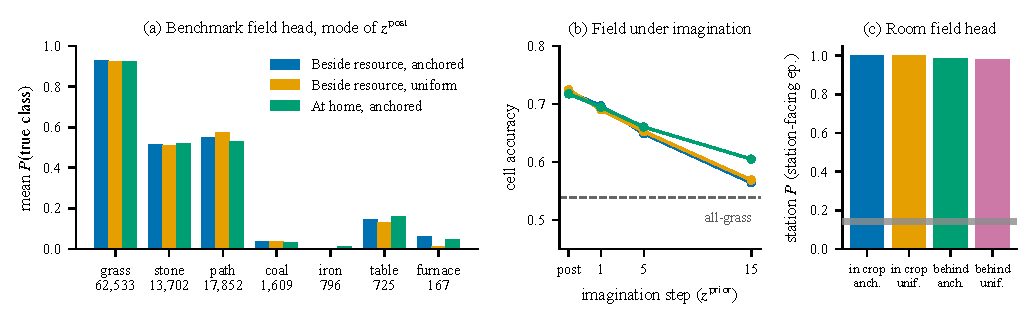
\includegraphics[width=\linewidth]{field_head.pdf}
  \caption{(a) Mean probability of the true class per material on the benchmark, with the number of probe cells under each label. (b) Cell accuracy of the field decoded from the posterior (``post'') and from the mode of $\zprior$ after 1, 5, and 15 imagined steps, against predicting grass everywhere (dashed). (c) In the room, the probability of the station on the station cells of a station-facing demonstration, for each of the four models; the gray band is the range of the benchmark's crafting-table probability from panel (a).}
  \label{fig:field}
\end{figure}

\paragraph{Under imagination.}
The actor is trained on the field decoded from $\zprior$, so the relevant question is what survives a rollout.
\Cref{fig:field}(b) shows that accuracy is about 70\% one step into imagination, then falls to 65--66\% at five steps and 56--61\% at fifteen, the length of an imagined training rollout, against the \FieldBaseline\% grass floor.
Stone and path recall fall with it, while grass stays near 0.8, so by the end of the horizon the predicted field has drifted toward grass.
The station is not recovered: table recall is 0.08 at step 15 in all three runs (\cref{tab:prior} in \cref{app:extra}).
These rollout scores cover 3,465 cells per step, of which only 17--25 are table and 3--6 furnace, so the station recalls under imagination are coarse.
The decoded frames of these rollouts are dark and low in contrast (\cref{fig:openloop}); we read the field numbers, not the images.

\subsection{Room: the station is named}

In the room the same probe gives a different answer (\cref{fig:field}(c), \cref{tab:room-probe}).
All four models reach material accuracy 1.0 on both demonstrations, station recall 1.0, and no false station cells.
On the station-facing demonstration the models trained in that pose assign the station a mean probability of 1.000, and the models trained facing away assign 0.986 and 0.981.
Under imagination from the first frame of the hold, the field stays correct for 15 steps in the pose each model trained on.
The two models trained facing away still predict the station one step into an imagined station-facing hold and lose it by step five; the models trained facing the station keep it through step 15.
So in the room, but not on the benchmark, the latent states where the station is.
